
\begin{frame}[fragile,label=x86ex1]{x86 encoding example (1)}
    \begin{itemize}
    \item \lstinline|pushq %rax| encoded as {\tt 50}
        \begin{itemize}
        \item 5-bit opcode {\tt 01010} plus 3-bit register number {\tt 000} \\
        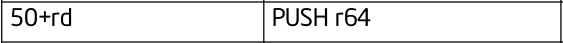
\includegraphics[width=0.4\textwidth]{../x8664-encoding/intel-manual-push-ex1}
        \end{itemize}
    \item \lstinline|pushq %r13| encoded as {\tt 41 55}
        \begin{itemize}
        \item {\tt 41}: REX prefix {\tt 0010} (constant), w:{\tt 0}, r:{\tt 0}, s:{\tt 0}, b:{\tt \color{blue!80!black}{1}}
        \item w = {\tt 0} because push is never 32-bit in 64-bit mode
        \item {\tt 55}: 5-bit opcode {\tt 01010}; 3-bit reg \# {\tt \color{green!80!black}{101}}
        \item 4-bit reg \# {\tt \color{blue!80!black}{1}\color{green!80!black}{101}} = 13
        \end{itemize}
    \end{itemize}
\end{frame}

\begin{frame}[fragile,label=x86ex2]{x86 encoding example (2)}
    \begin{itemize}
    \item \lstinline|addl 0x12345678(%rax,%rbx,2), %ecx|
    \item {\tt 03}: opcode --- add r/m32 into r32 
        \begin{itemize}
        \item
            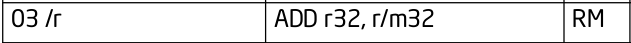
\includegraphics[width=0.4\textwidth]{../x8664-encoding/intel-manual-addl-ex1.png}
            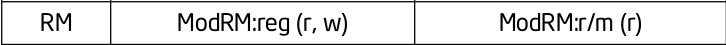
\includegraphics[width=0.4\textwidth]{../x8664-encoding/intel-manual-addl-ex2.png}
        \end{itemize}
    \item {\tt 8c}: ModRM: mod = {\tt 10}; reg = {\tt 001}, r/m: {\tt 100}
        \begin{itemize}
        \item reg = {\tt 001} = {\tt \%ecx} (table)
        \item SIB byte + 32-bit displacement (table)
        \end{itemize}
    \item {\tt 58}: SIB: scale = {\tt 01}, index = {\tt 011}, base = {\tt 000}
        \begin{itemize}
        \item index {\tt 011} = {\tt \%rbx}; base {\tt 000} = {\tt \%rax};
        \end{itemize}
    \item {\tt 78 56 32 12}: 32-bit constant {\tt 0x12345678}
    \end{itemize}
\end{frame}

\begin{frame}[fragile,label=x86ex3]{x86 encoding example (3)}
    \begin{itemize}
    \item \lstinline|addq 0x12345678(%r10,%r11,2), %rax|
    \item {\tt 4b}: REX prefix {\tt 0100}+w:{\tt \myemph<2>{1}}, r:{\tt \textcolor{violet!80!black}{\myemph<3>{0}}}, s:{\tt \textcolor{blue!80!black}{\myemph<4>{1}}}, b:{\tt \textcolor{green!80!black}{\myemph<5>{1}}}
    \item {\tt 03}: opcode --- add r/m64 to r64 (with \myemph<2>{REX.w})
    \item {\tt 84}: ModRM: mod = {\tt 10}; reg = {\tt 000}, r/m: {\tt 100}
        \begin{itemize}
        \item reg = {\tt \textcolor{violet!80!black}{\myemph<3>{0}}000} = \%rax
        \item SIB byte + 32-bit displacement (table)
        \end{itemize}
    \item {\tt 5a}: SIB: scale = {\tt 01}, index = {\tt 011}, base = {\tt 010}
        \begin{itemize}
        \item with REX: index = {\tt \textcolor{blue!80!black}{\myemph<4>{1}}011} (11), base = {\tt \textcolor{green!80!black}{\myemph<5>{1}}010} (10)
        \end{itemize}
    \item {\tt 78 56 32 12}: 32-bit constant {\tt 0x12345678}
    \end{itemize}
\end{frame}

\begin{frame}[fragile,label=x86ex4]{x86 encoding example (4)}
    \begin{itemize}
    \item \lstinline|movq %fs:0x10,%r13|
    \item {\tt 64}: FS segment override
    \item {\tt 48}: REX: {\tt w}: 1 (64-bit), {\tt r}: \textcolor{violet!80!black}{\tt \myemph<2>{1}}, {\tt s}: \textcolor{blue!80!black}{\tt \myemph<3>{0}}, {\tt b}: \textcolor{green!80!black}{\tt \myemph<4>{0}}
    \item {\tt 8b}: opcode for MOV memory to register
    \item {\tt 2c}: ModRM: mod = {\tt 00}, reg = {\tt 101}, r/m: {\tt 100}
        \begin{itemize}
        \item with REX: reg = {\tt \textbf{\textcolor{violet!80!black}{\myemph<2>{1}}}101} [\%r12]; r/m = {100} (SIB follows)
        \end{itemize}
    \item {\tt 25}: SIB: scale = {\tt 00}; index = {\tt (\textcolor{blue!80!black}{\myemph<3>{0}})100}; base = {\tt (\textcolor{green!80!black}{\myemph<4>{0}})101}
        \begin{itemize}
        \item no register/no register in table
        \end{itemize}
    \item {\tt 10 00 00 00}: 4-byte constant {\tt 0x10}
    \end{itemize}
\end{frame}


